\subsection{ETH measurements with block mining period 2s.}

\textit{Author: Jacek Janczura} \\
Throughput was measured consequently with the two previously aforementioned definitions. In the Fig.\ref{fig:throughput1} throughput was measured as average number of transactions in a block divided by the block frequency and in the Fig.\ref{fig:throughput2} throughput was measured using our own formula.
 
\begin{table}[!h]
\centering
\begin{tabular}{l|l|l|l|l|}
\hline
\multicolumn{1}{|l|}{\textbf{tx}} & \textbf{tbn-t0 {[}s{]}} & \textbf{Thr. alt. {[}tx/s{]}} & \textbf{Avg(tx/block)} & \textbf{Thr. {[}tx/s{]}} \\ \hline
\multicolumn{1}{|l|}{\textit{10}} & \textit{2.69} & \textit{3.72} & \textit{10} & \textit{5} \\ \hline
\multicolumn{1}{|l|}{\textit{100}} & \textit{2.79} & \textit{35.80} & \textit{100} & \textit{50} \\ \hline
\multicolumn{1}{|l|}{\textit{1000}} & \textit{10.67} & \textit{93.72} & \textit{200} & \textit{100} \\ \hline
\multicolumn{1}{|l|}{\textit{10000}} & \textit{99.82} & \textit{100.18} & \textit{204.08} & \textit{102.04} \\ \hline
\multicolumn{1}{|l|}{\textit{100000}} & \textit{1711.73} & \textit{58.42} & \textit{117.1} & \textit{58.55} \\ \hline
\multicolumn{1}{|l|}{\textit{489290}} & \textit{8935.53} & \textit{54.76} & \textit{109.53} & \textit{54.765} \\ \hline
& \textbf{AVG} & \textit{\textbf{57.77}} & \textit{\textbf{123.45}} & \textit{\textbf{61.73}} \\ \cline{2-5}
& \textbf{AVG filtered} & \textit{\textbf{76.77}} & \textit{\textbf{157.68}} & \textit{\textbf{78.84}} \\ \cline{2-5}
\end{tabular}
\caption{ETH: Throughput measurement results. Block mined every 2s.}
\label{table:2}
\end{table}
 
Table \ref{table:2} presents the results of the throughput measurements. In ethereum private blockchain we have observed that in case of lower blockchain load ($tx < 10000$) throughput is in average around 100 transactions per second and the average number of transactions in a block is then at the level of around 200 tx/block. Unfortunately in case of higher blockchain load  throughput falls to the level of 50 tx/s and stays on that level even in a really overloaded blockchain.
 
 
 
The results from measuring the throughput in both ways Fig.\ref{fig:throughput1} and Fig.\ref{fig:throughput2} results in similar numbers - average filtered throughput between 75-80 tx/s.
 
\begin{figure}[!h]
    \centering
    %\captionsetup{justification=centering}
    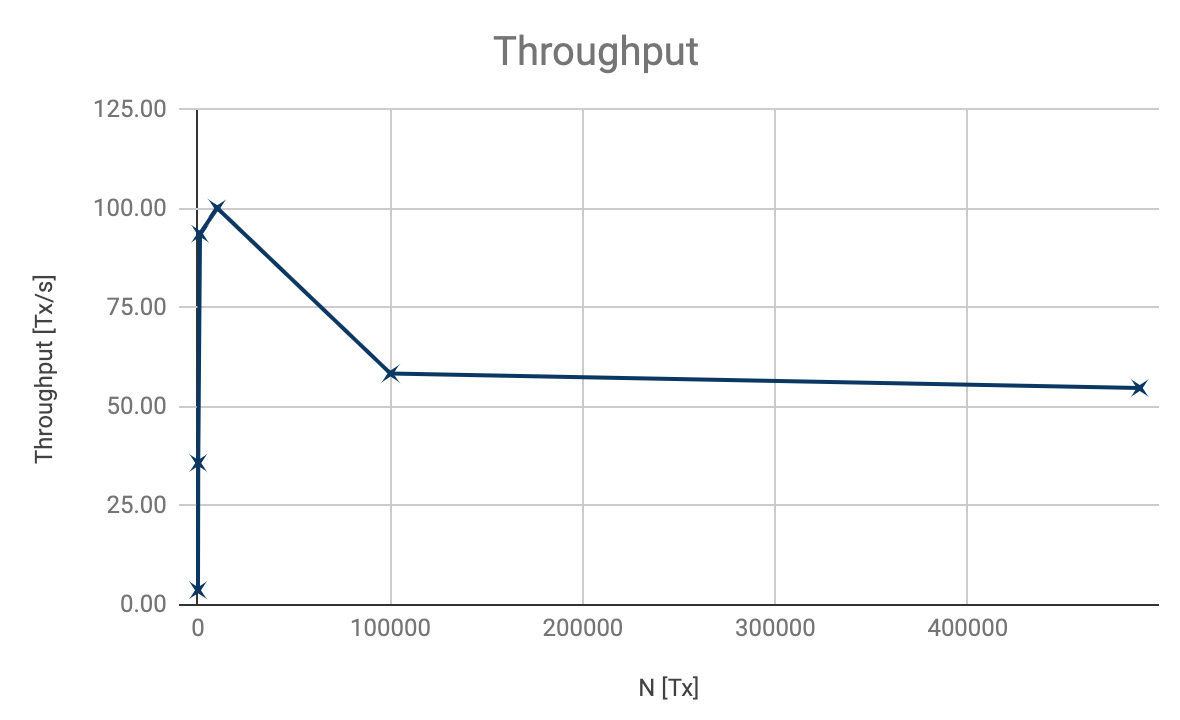
\includegraphics[width=0.75\textwidth]{img/Throughput_ETH.png}
   \caption{ETH: Throughput as average number of transactions in a block divided by the block frequency}
   \label{fig:throughput1}
\end{figure}
 
\begin{figure}[!h]
    \centering
    %\captionsetup{justification=centering}
    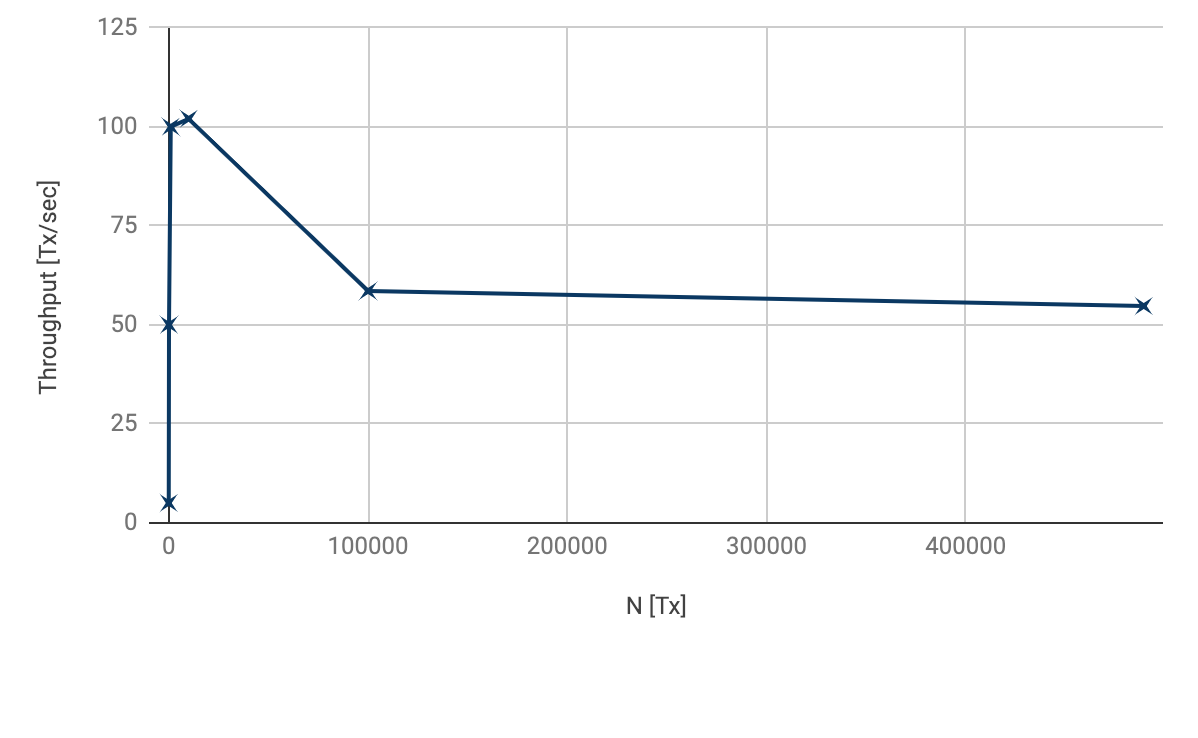
\includegraphics[width=0.75\textwidth]{img/Throughputalt.png}
   \caption{ETH: Throughput as total number of transactions divided by time from submitting the first transaction until mining the last block}
   \label{fig:throughput2}
\end{figure}
 
In Fig. \ref{fig:txbig} we present the number of transactions per block. It is clearly visible that for  higher load average $tx/block$ stays in the level of 100 ts/block. We have data for 1 million transactions as well. The results are the same as for 100 000 but the chart is less clear. That is why we have decided to present this one.
 
\begin{figure}[!h]
    \centering
    %\captionsetup{justification=centering}
    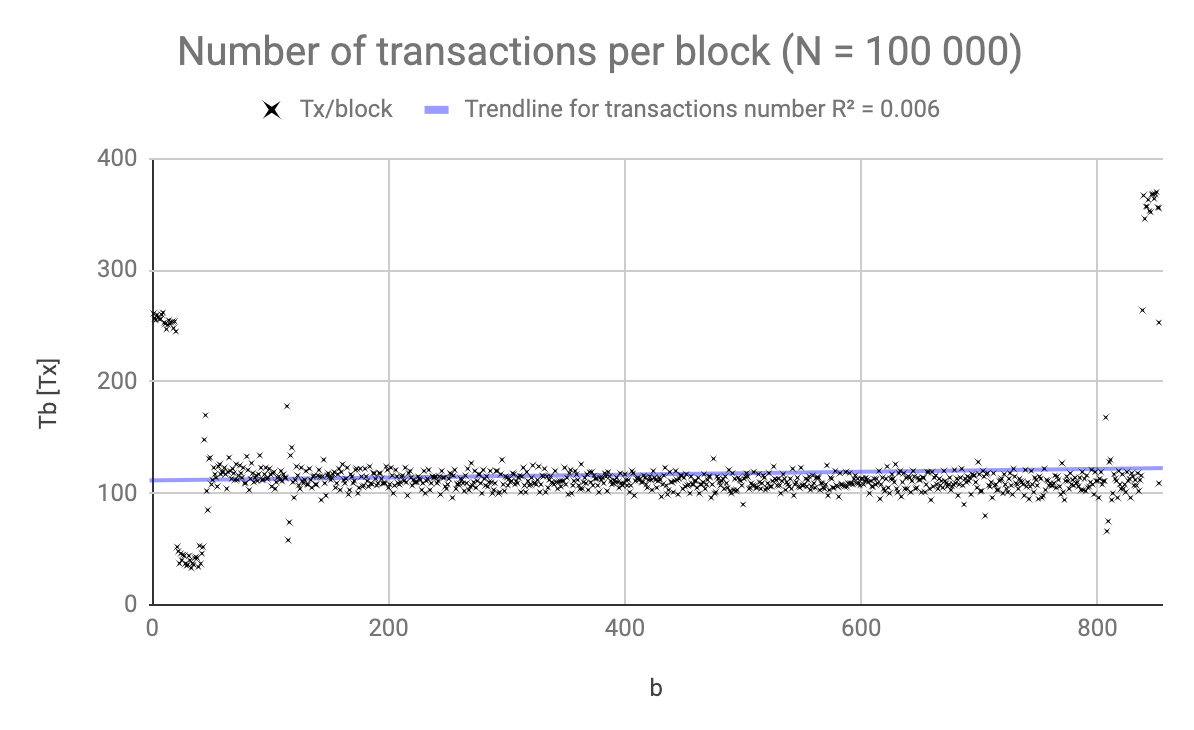
\includegraphics[width=0.75\textwidth]{img/txmed.png}
   \caption{ETH: Block capacity in a higher blockchain load conditions}
   \label{fig:txbig}
\end{figure}
 
What is interesting is, that we wanted to observe the drop in the block capacity. This drop is presented in Fig. \ref{fig:txsmall}. We think that this might be the result of an internal blockchain balancing but we could not proof that. That is why this problem needs further research.
 
\begin{figure}[!h]
    \centering
    %\captionsetup{justification=centering}
    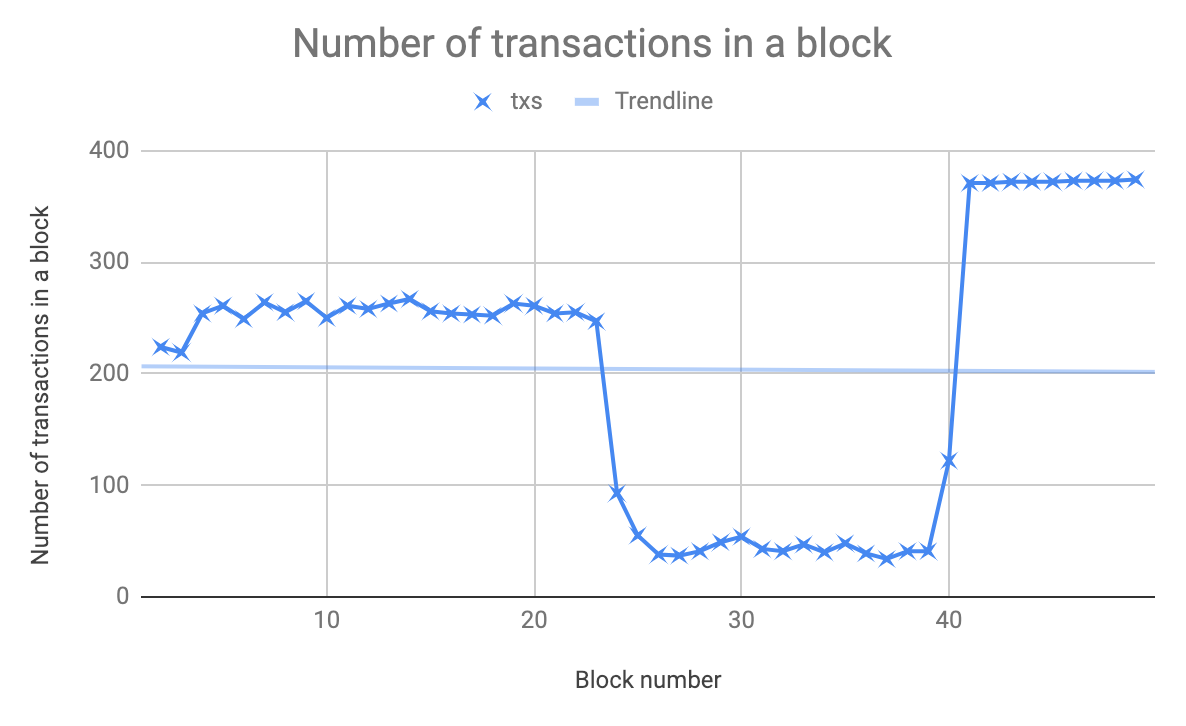
\includegraphics[width=0.75\textwidth]{img/TxNumperBlockSmall.png}
   \caption{ETH: Drop in the block capacity}
   \label{fig:txsmall}
\end{figure}